
\chapter*{About this project}
\paragraph{Abstract:}
"Tech will transform from something we actively use to a more seamless integrated experience that is ‘on’ all the time." Daniel Baek, Co-founder of Nodes~\cite{nodes}. This paper proposes a new phone application that consists of the most important activities and features in demand for third level students around in Ireland. Feature's that can be accessed 24/7 and effortlessly by any user. The aim of this project was to create a suitable application that would benefit users in all aspects of their studies. Studies show that each household has an average of six devices connected to the internet. These consist of smart phones, laptops, computers and some household appliances. It was decided that this project would be developed for the most portable device held by users, mobile phones. Current deals with network vendors also allow the user to be connected to the internet through 3G or 4G technologies. All colleges maintain their own network for students also, this means that our application can be downloaded and used at all times.

\paragraph{Authors:}
This project was developed by two 4th year development students, Aaron Flanagan and Ciaran Brennan, as part of our Bachelors of Science honours degree in Applied Software Development.

\chapter*{Acknowledgements:}
We would like to acknowledge and thank Damien Costello for supervising this project. His expert advice and support helped guide this project to completion. We would also like to acknowledge the Department of Computer science and Applied Physics for making this possible and helping us by providing support and any tools that were needed during the development.

\chapter{Introduction}
The original idea for this project was to develop a facial recognition music application. The application would begin by capturing an image of the users face and running a mood capturing algorithm to determine the users mood, and it would then generate a music file list based on the users mood. This projects foreground was going to include an animated graphical user interface through the use of the JavaFX library made available by Oracle ~\cite{javafx}. The background was running a facial detection program that was described by the OpenCV Team~\cite{opencv}. This algorithm was going to built upon to include facial recognition as it only produced facial detection on screen by drawing shape around the users face, but this needed a feature extraction algorithm to complete it and that's when the idea discovered a problem that could not be solved. We had to make a decision,  either change language or change the idea for the project. Since the developers are both competent in Java we decided to change the project rather than change the language. The reason we could not continue in Java was because we spent weeks of research and study involving different approaches of facial recognition and feature extraction it was found that there was no Java binding libraries to OpenCV or resources that we could use. After a week of searching nothing was found that could help us, but because it was still early into the year the project idea had to be changed as to avoid further problems and time delay.

It was October/November and the project was still at the beginning, GMIT hosted a hackathon for other colleges with software development courses to develop a project over a two day period. This time was used to explain the problem and come up with a new idea and build upon it until a clear project goal and list of possible features where decided on. Damien Costello was informed about the problem and advised that the project idea could be changed while it was still possible, he was understanding and suggested a few ideas of projects to think about and do some research into. Out of those ideas came the student application idea, the development of an integrated mobile application solely for the purpose of third level students. He suggested doing something in augmented reality. It was thought upon and we decided that the projects goal would be to build an application for students that includes, but not limited to, the augmented reality section in the form of navigation around the college in addition to using the Google maps API for the use of Google maps within our application. A list was constructed of things that tend to be a problem for students and academic staff managing multiple years of students. Further research was done into the market to see what was already done and available. Many developers have developed applications with timetables or notes for your phone screen but none could be found that contained all of these sections integrated into one application, or that where just institution specific. After deciding what kind of application was to be built, the platform technology had to be chosen, this included research into the available systems. Finally a list of features had to be narrowed down to include in the project, what features would be more beneficial and would provide better context to the final application.

Further into this report will contain a breakdown and give an in-depth explanation to how the project was approached and developed, the different software and technologies used, an evaluation of the final product and notes taken by the developers about each feature and where they can be improved and why. The following sections will be discussed about the application:
\begin{itemize}
\item Methodology: This explains the production approach taken to developing the individual features of the application and how they were developed within the project time limit.
\item Technology review: This section discusses the various technologies used, both hardware and software. It explains how the project uses each component and gives an explanation to why this particular system/software was used and what is was used for.
\item System design: This section gives a breakdown of the projects architecture. How the system is built and how everything fits together.
\item System Evaluation: This section evaluates the finished project and provides a list of improvements that can be made.
\item Conclusion: The final discussion about the project and evaluation of its finished state. Each section will be briefly concluded and its main points will be stated.
\end{itemize}

This project can be found on GitHub under the name AaronFlanagan20 or CiaranB1992: https://github.com/AaronFlanagan20/CollegeEssentialsApp.
The repository contains a small ReadMe file about how to download and run the application. The repository holds all the classes and native android files created and used by Android Studio to compile and run the project. Your computer or laptop must support virtualization, this can be checked by attempting to install Intel's hardware accelerator software or by checking in the task manager of your machine. If your machine does not support it, you will be unable to run the emulator, instead you must plug in an android device with the developer options enabled.

\chapter{Methodology}
\section{Planning}
The first step of the project was planning everything that had to be done. This included when to hold meetings, what software to use for the development, what methodology to approach it with and how to test it appropriately. The first task finished was the creation of a project work flow to create a timely estimate of how long each feature will need and take into account other responsibilities the developers might have with other projects and reports. The project work flow or Gantt chart, was developed to show everything that needed to be done. It leaves out the section that assigns each individual developer to a particular area or feature because the list of features was not particularly large enough to scale out seven months of development and it was more beneficial to work as a pair due to the methodology taken. See Figure 2.1.

\section{Software Methodology}
Next was the decision of which methodology to pursue. It was decided this project would be developed based on agile methodologies. "Agile methodology is an alternative to traditional project management, typically used in software development. It helps teams respond to unpredictability through incremental, iterative work cadences, known as sprints "~\cite{agile}. The traditional waterfall approach was not taken due to its limitations put on each phase of the project. Each section had to be completed in sequential order and time did not permit backtracking if a problem arouse. Instead an incremental approach was taken. Both developers met up to discuss which feature to work on and to begin working on it by researching previously made work and reading through the Android documentation to find relative libraries available. This meant that each feature could be developed no matter how long it took to finish and different approaches could be taken. One feature may have taken a week at most to develop allowing  more time to improve it, while the next might have taken a month to complete. It also allowed more research and the ability to develop up-to date documentation and code during the development of each feature. If the code was re-factored or a different approach was taken that differed from the pre-determined plan specified at the beginning of this project, the developers where free to make the change and it was documented. During the development of that feature however, an iterative approach was taken. Each developer would plan, develop and test the feature and resort back to the original documentation to evaluate it. The same process would be taken again until the feature was eventually finished. At the end of each features cycle a meeting was held to discuss and evaluate it with the supervisor. These consisted of ideas on how to improve it or how to begin on the next. 

\section{Testing}
At the end of a features cycle, some testing was performed before moving on. This project used three forms of testing. The first form of testing is Gradle, that is built into Android Studio. Gradle is a project build automation tool used to compile, test and run a native Java project and slow done build time and code freeze ups ~\cite{gradle}. It complies and runs the project within Android studio. Next used was CircleCI, CircleCI is a cloud platform used for continuous integration. Every time a commit was pushed up to the repository using git, CircleCI would pull down the code from GitHub and run a selection of tests on the new changes. If it passed the test the commit would integrate with the rest of the project on GitHub, if failed it would not be integrated until the problem was fixed via another commit to update and fix the changes or revert the commit to remove the changes. Finally the developers wrote tests for the application using JUnit. JUnit is "A unit testing framework which is a central element of the Extreme Programming (XP) testing practice."~\cite{junit} JUnit was used to test the actions of components in the application to see if they performed the way they were supposed to, example if a pop-up box is meant to display on the press of a button. 
\begin{figure}
	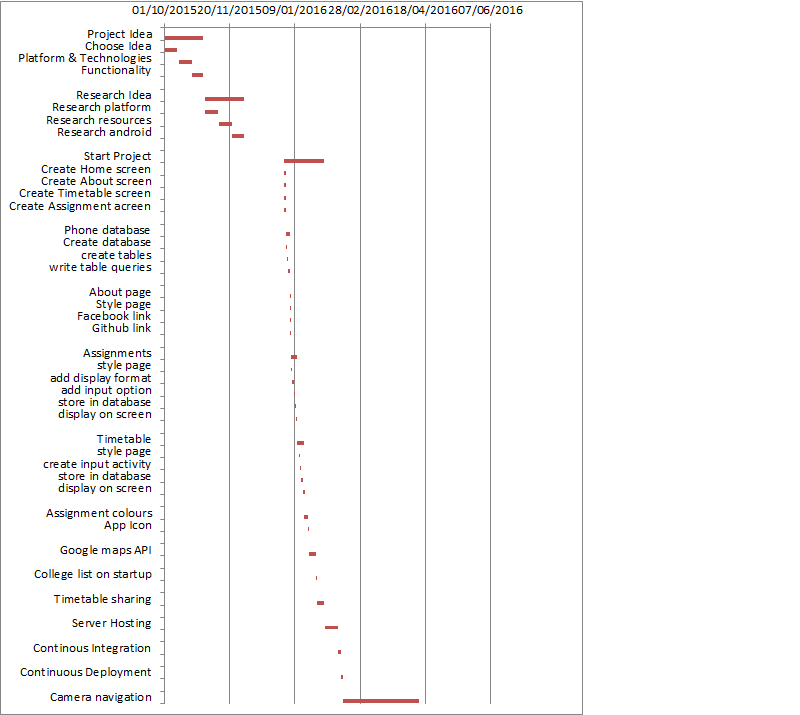
\includegraphics{img/gannt.png}
	\caption{Project Work Flow}
\end{figure}

\chapter{Technology Review}
About seven to ten pages.
\begin{itemize}
\item Describe each of the technologies you used at a conceptual level. Standards, Database Model (e.g. MongoDB, CouchDB), XMl, WSDL, JSON, JAXP.
\item Use references (IEEE format, e.g. [1]), Books, Papers, URLs (timestamp) – sources should be authoritative. 
\end{itemize}

\section{XML}
Here's some nicely formatted XML:
\begin{minted}{xml}
<this>
  <looks lookswhat="good">
    Good
  </looks>
</this>
\end{minted}

\chapter{System Design}
\section{Server connection}
The system design is fairly straight forward. The first page is the CollegeSelection activity. This consists of a ListView object that contains a list of colleges in the country. Once a college is selected the application creates a database with the college's name using SQLite and makes a connection to Heroku's PostgreSQL database to retrieve the binary of image of chosen college to display it on the HomeScreen activity. In Android they use a UIThread to handle all the on screen displays and actions, this is the main thread. However they do not allow networking actions on this thread, a separate thread must be started and ran in the background. This was not possible because the Heroku connection need to be made to continue on. To tackle this problem the main UIThread is forced to wait for the connection thread to finish, this is not the best way to handle the problem but it served as a temporary solution until another can be found. The connection was made as follows:

\begin{minted}{java}
try {
	connect.start();//start thread
	connect.join();//forcing UI thread to wait until connection is complete
}catch (InterruptedException e){
	e.printStackTrace();
}
\end{minted}

The connect thread created a Heroku connection which in turn called the connect method from it's constructor. The Thread.join() statement is forcing all other Threads to wait until it has finished. Below are two screen-shots of the application, and Figure 4.3 describes the flow of events that take place.

\begin{figure}[!b]
	\begin{minipage}[b]{0.47\textwidth}
		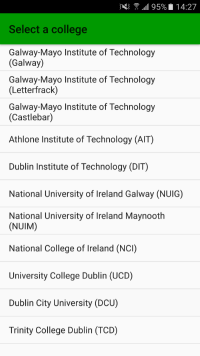
\includegraphics{img/collegeselection.png}
		\caption{CollegeSelection activity}
	\end{minipage}
	\hfill
	\begin{minipage}[b]{0.47\textwidth}
		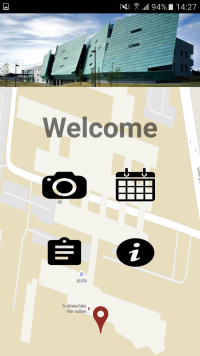
\includegraphics{img/homescreen.png}
		\caption{HomeScreen activity}
	\end{minipage}
\end{figure}

\begin{figure}[!hb]
	\centering
	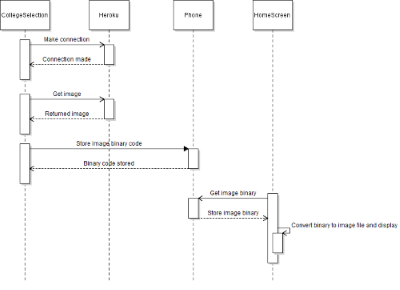
\includegraphics{img/heroku-connection.png}
	\caption{Connection to Heroku sequences}
\end{figure}

\clearpage
\section{Database Technology}
"SQLite is a software library that implements a self-contained, serverless, zero-configuration, transactional SQL database engine. SQLite is the most widely deployed database engine in the world"~\cite{sqlite}. This database management system is independent and available on all mobile platforms. It uses the database query language SQL to insert, delete, update and query database tables made on the users phone and stores information relevant to the application. In Android two objects are used to create and maintain them, SQLiteDatabase exposes methods to manage a SQLite database and SQLiteHelper is a helper class to manage database creation and version management. The application contains three stand-alone tables: Timetable, Assignment and Markers. Timetable contains three columns: module name, room number and teacher name, assignment contains two columns: subject name and the due date and Marker contains three columns: marker name, the longitude and latitude of the selected place in the Google maps section.\newline

\begin{figure}[h]
	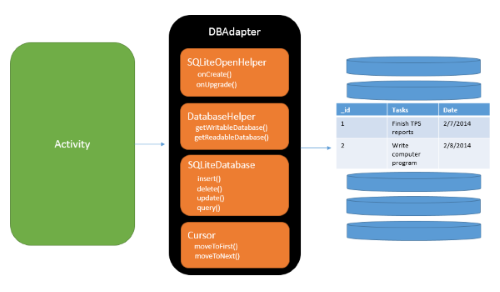
\includegraphics{img/Android-SQLite-Overview.png}
	\caption{SQLite objects}~\cite{using-the-sqlite-database}
\end{figure}

\section{Timetable activity}
The Timetable class of the project creates a screen of TextView objects in the form of columns and rows that represent the days Monday-Friday and times 9:00am - 6:00pm. By clicking a TextView box or by clicking the plus icon in the top right corner a new activity begins to enter in the subject, room, teacher, day and time. This all gets stored in the Timetable table of the database. On creation the class loops through the parent layout collects all TableRows in it, it then loops through every TableRow and selects all the TextView's each of them contain, it creates a temporary TextView object sets it's allowed boundaries and calls the paintTimetable() method.

\begin{minted}{java}
private void getAllTextViews() throws Exception {
 for(int i = 1; i < layout.getChildCount(); i++){//loop through parent layout
  if(layout.getChildAt(i) instanceof TableRow) {//get every child that's a TableRow
   TableRow row = (TableRow) layout.getChildAt(i);//create temp TableRow
   for(int x = 1; x < row.getChildCount(); x++){//loop through temp TableRow
    if(row.getChildAt(x) instanceof TextView){//get every TextView in temp TableRow
	 TextView temp = (TextView) row.getChildAt(x);//set child to temp
	 temp.setOnClickListener(this);
	 temp.setMaxWidth(temp.getWidth());//set size's
	 temp.setMinWidth(temp.getWidth());		
	 temp.setMaxHeight(temp.getWidth());
	 temp.setMaxHeight(temp.getWidth());		
	 paintTimetable(temp);//fill child with details stored in database
    }
   }
  }
 }
}
\end{minted}

This method takes the TextView as an argument, calls the getIDName() method and retrieves the id in the form of day-time and checks the database for any information it may contain. In the unlikely case the view does not have an id it wil just return a blank string. A Cursor object is used in Android to loop through the database and store string variables of the data in each column. A check is done to see if the TextView's dy and time has any information stored under it and if so it sets the text to it and paints it on screen within the TextView's specified boundaries.
\pagebreak

\begin{minted}{java}
private void paintTimetable(TextView view) throws Exception {
 String id = getIDName(view, R.id.class).toLowerCase();//pass in an object and get it's id
 String[] search = id.split("_");//split day from time (MON) _NINE
 
 Cursor c = ad.returnTimetableData();//return all data from  database
 
 if(c.moveToFirst()){
  do{
  // Collect each rows data
  String module = c.getString(0);
  String room = c.getString(1);
  String teacher = c.getString(2);
  String day = c.getString(3);
  String time = c.getString(4);
 
   if(day.equals(search[0]) && time.equals(search[1])){// if day = "mon" and time = "nine"
    view.setText(String.format("%s\n%s\n%s", module, room, teacher));//paint details on screen
   }
 
  }while (c.moveToNext());//move to next row in database
 }
}
\end{minted}

\begin{figure}[b]
	\begin{minipage}[h]{0.4\textwidth}
		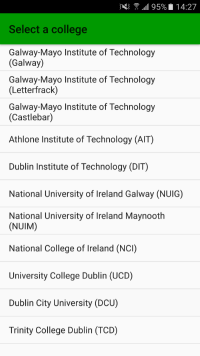
\includegraphics{img/collegeselection.png}
		\caption{CollegeSelection activity}
	\end{minipage}
	\hfill
	\begin{minipage}[h]{0.4\textwidth}
		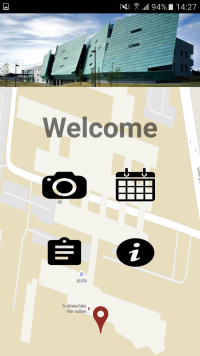
\includegraphics{img/homescreen.png}
		\caption{HomeScreen activity}
	\end{minipage}
\end{figure}

\chapter{System Evaluation}
\section{Memory and Server}
The database management system used is SQLite. This was chosen because all mobile platforms support it. This enables the phone to have a certain degree of control on what information to get when needed. Once the user selects a college on start-up of the application a database with the college name is created on the phone allowing each selection to have its own database to store a timetable, assignments and custom google map markers the user may have placed. The database model is quite simple. It stores two tables Timetable and Assignment. The Timetable activity contains three columns room, teacher and subject, while the assignment activity contains two, subject and due-date. With information stored in multiple databases the applications overall size averages around 27.5 mb, which compared to a huge application likes Facebook's social network it is miniscule because Facebook's is currently at 365mb. 
A connection is also made to Heroku's PostgreSQL database to pull down an image of the college stored and all the co-ordinates needed for the navigation section. It was done this way to save memory on the phone. Instead of each database per college storing the image and wasting memory it retrieves the binary of said image and re-converts it to a bitmap from the main screen every time the application is used and places it on screen. To do this a separate project was made to act as the Heroku maintenance code of the database, also using java. This code is used to test the pushing and pulling of information to the server. Once everything is pushed up it never has to be done again, but the code is then integrated into the project to deal with retrieving the image.

\section{Universality}
A decision to make the application universal was made during the development. All students can use the timetable and assignment features and the navigation section will be constantly updated to allow other various colleges to use it. However at the moment the application is only accessible to Android users. Android was chosen because it's native language is java and this is well-known by the developers. However the initial intentions of the project were for it to be available on all platforms. Different technologies exist that allow the application to be complied cross-platform to the IOS operating system for IPhone and Microsoft Windows operating system for Microsoft phones, but this was not accomplished because time ran out. The overall structure of the project will be concrete regardless of the operating system because of the platform neutral technologies chosen. The chosen database explained previously in the technology review of this report is SQLite. SQLite is supported by all mobile platforms as a database choice. The syntax of all the internal queries made in the application will remain the same. The same concept applies to the college selection, as previously explained Heroku's PostgreSQL database is entirely independent from the applications architecture. The only difference being the driver that enables the connection on each platform. Android uses java's JDBC driver to connect. This driver will be of no use to the other platforms because IOS is written in either Objective-C or Swift using the ODBC driver, and Windows is written using C-Sharp and uses the ADO.NET driver. This means each operating system specific deployment of the project will need to have its own driver included and the syntax within the CollegeSelection class of the project will have to change slightly to replace the JDBC driver with the new one. Each language uses it's predefined driver in order to make a connection to Heroku's database and retrieve information based on an SQL query the application makes. This was done so the phone doesn't waste memory storing information on all colleges. See Figure 5.1.
In conclusion the application is universal due to the number of colleges and universities that can use it. It can also be easily transformed to be cross-platform with some minor changes needed to one section of code that makes the initial connection.

\pagebreak\section{Improvements}
Each section of the application has areas where improvements could be made if more time was available. Below is a list of possible improvements that can be made in the future for the application in general and each individual section. 
\begin{itemize}
	\item Application: A priority queue added to handle threads because the current implementation creates a lag in the connection.
	\item Application: Add in an instant messenger section for students to talk to one another about their timetables and current assignments.
	\item Application: Add a section that users can personalize it to their preference.
	
	\item Camera navigation: More colleges and universities in the country can be added to the list.
	\item Camera navigation: Better graphics can be used for augmented reality.
	\item Camera navigation: More responsive software to deal with multiple locations within the geo-fencing area.
	\item Camera API: A swap from the deprecated Camera API to the new camera API made available for newer Android SDK's. 
	
	\item Assignment: The ability for users to share assignments across platforms with each other.
	\item Assignment: Section for lecturers to upload assignments and the users can just enrol to that assignment.
	
	\item Timetable: The ability for users to share timetables with each other.
	\item Timetable: Section for colleges to upload timetables automatically and users can download it.
	\item Timetable: Colour code each section of the timetable.
	
	\item Google Maps: Option to view each individual floor of a building being seen.
	\item Google Maps: Provide directions from current location to a marker chosen by the user.
\end{itemize}

\begin{figure}
	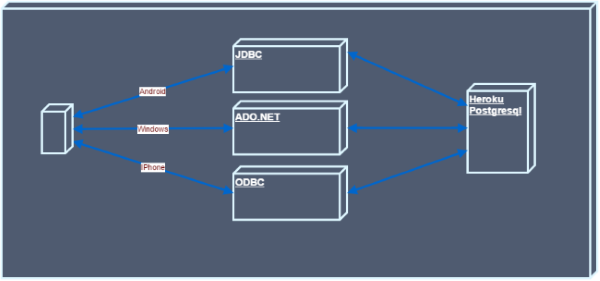
\includegraphics{img/connection-diagram.png}
	\caption{Phone Driver Diagram}
\end{figure}
\chapter{Conclusion}
About three pages.

\begin{itemize}
\item Briefly summarise your context and ob-jectives (a few lines).
\item Highlight your findings from the evalua-tion section / chapter and any opportuni-ties identified.
\end{itemize}

